\documentclass[a4paper,12pt]{article}
\usepackage{graphicx}  % For including logos or images
\usepackage{titling}   % For better control of title formatting
\usepackage{amsmath,amssymb}
\usepackage{tikz}
\usetikzlibrary{shapes.gates.logic.US, positioning}
\usepackage{enumitem}
\usepackage{amsfonts}
\usepackage{booktabs}
\usepackage{array}

\begin{document}

\begin{titlepage}
    \centering
    
    \vspace{1cm}
    
    {\Huge \textbf{Group Assignment-01}}\\[1cm]
    {\LARGE EE1201: Digital Systems}\\[1.5cm]
    
    \rule{\linewidth}{0.5mm}\\[0.5cm]
    {\Large \textbf{Submitted by}}\\[0.3cm]
    {\large Group-3}\\[1cm]
   
    {\Large \textbf{Submitted to}}\\[0.3cm]
    {\large Siva Vanjari Sir}\\
    {\large Indian Institute of Technology Hyderabad}\\[1.5cm]
    
    \rule{\linewidth}{0.5mm}\\[1.5cm]
    {\large \textbf{Date of Submission:} \today}\\[2cm]
    
    \vfill

\end{titlepage}

\newpage
\section{Intro To Digital Systems}
\subsection{Role of Digital Systems}
\begin{itemize}
    \item Digital systems are integral to various fields, including communication, business, traffic control, medical applications, weather monitoring, and scientific research.
    \item They are embedded in everyday devices such as digital telephones, televisions, cameras, and handheld touchscreen devices.
\end{itemize}

\subsection{Binary Representation in Digital Systems}
\begin{itemize}
    \item Digital systems operate on discrete elements of information, represented using \textbf{binary digits (bits)}—0 and 1.
    \item Groups of bits, called \textbf{binary codes}, represent numbers, characters, and symbols.
    \item The decimal number system can be converted into binary, where each number is expressed using a sequence of bits (e.g., $7_{10} = 0111_2$).
\end{itemize}

\subsection{Core Components of a Digital Computer}
\begin{itemize}
    \item \textbf{Memory Unit}: Stores programs, data, and intermediate results.
    \item \textbf{Central Processing Unit (CPU)}: Executes arithmetic, logic, and data processing operations.
    \item \textbf{Input/Output Devices}: Allow data entry (e.g., keyboards, touchscreens) and result display (e.g., printers, monitors).
    \item \textbf{Communication Unit}: Enables data exchange through networks, such as the Internet.
\end{itemize}

\subsection{Binary Logic and Digital Circuits}
\begin{itemize}
    \item Digital circuits process binary signals using \textbf{logic gates} (AND, OR, NOT, etc.).
    \item \textbf{Flip-flops} store binary data and are used in memory and sequential circuits.
\end{itemize}

\subsection{Advantages of Digital Systems}
\begin{itemize}
    \item \textbf{High Speed}: Modern digital circuits perform operations at millions of cycles per second.
    \item \textbf{Programmability}: Many digital devices can be reprogrammed for different tasks, making them versatile.
    \item \textbf{Reliability}: Error-correcting codes ensure accurate data storage and transmission.
    \item \textbf{Cost Efficiency}: Advances in \textbf{integrated circuit (IC) technology} reduce manufacturing costs while increasing performance.
\end{itemize}

\subsection{Quantization of Data}
\begin{itemize}
    \item Digital systems process both inherently discrete data (e.g., payroll records) and \textbf{quantized} continuous data (e.g., temperature readings).
    \item \textbf{Analog-to-Digital Converters (ADCs)} transform continuous signals into digital form (e.g., in digital cameras).
\end{itemize}

\subsection{Digital System Design Using HDL}
\begin{itemize}
    \item Modern digital systems are designed using \textbf{Hardware Description Languages (HDLs)}, which describe circuit functionality in textual form.
    \item HDLs enable simulation, verification, and synthesis of digital circuits before fabrication.
    \item Proper HDL-based design ensures efficient and functional digital hardware.
\end{itemize}

\subsection{Conclusion}
\begin{itemize}
    \item Digital systems form the foundation of modern computing and information processing.
    \item Their ability to represent and manipulate binary data makes them highly efficient and widely used.
    \item Understanding binary representation, logic circuits, and digital design methodologies is essential for working with digital technology.
\end{itemize}

\newpage

\section{Binary Numbers }
\subsection{Decimal Number System (Base 10)}
A decimal number consists of digits from 0 to 9, with each digit's place value determined by powers of 10.
For example, the number 7392 can be expressed as:
\begin{equation}
  7 \times 10^3 + 3 \times 10^2 + 9 \times 10^1 + 2 \times 10^0
\end{equation}

\subsection{Number Systems and Radix (Base)}
A number system's radix (or base) determines the set of digits and the positional values of those digits:
\begin{itemize}
    \item \textbf{Decimal System (Base 10):} Uses digits 0-9.
    \item \textbf{Binary System (Base 2):} Uses only two digits: 0 and 1.
    \item \textbf{Octal System (Base 8):} Uses digits 0-7.
    \item \textbf{Hexadecimal System (Base 16):} Uses digits 0-9 and letters A-F.
\end{itemize}

\subsection{Binary Number System (Base 2)}
In the binary system, each digit is either 0 or 1 and is multiplied by a power of 2.
For example, converting $1100.11_2$ to decimal:
\begin{equation}
  (1 \times 2^3) + (1 \times 2^2) + (0 \times 2^1) + (0 \times 2^0) + (1 \times 2^{-1}) + (1 \times 2^{-2}) = 12.75_{10}
\end{equation}

\subsection{Octal Number System (Base 8)}
The octal system has eight digits (0 to 7). For example, converting $(127.4)_8$ to decimal:
\begin{equation}
  (1 \times 8^2) + (2 \times 8^1) + (7 \times 8^0) + (4 \times 8^{-1}) = 87.5_{10}
\end{equation}

\subsection{Hexadecimal Number System (Base 16)}
The hexadecimal system has sixteen symbols (0-9 and A-F). For example, converting $(B65F)_{16}$ to decimal:
\begin{equation}
  (11 \times 16^3) + (6 \times 16^2) + (5 \times 16^1) + (15 \times 16^0) = 46687_{10}
\end{equation}

\subsection{Powers of Two and Storage in Computers}
The binary system is widely used in computing. Common memory sizes:
\begin{itemize}
    \item $2^{10} = 1024$ bytes = 1 KB
    \item $2^{20} = 1,048,576$ bytes = 1 MB
    \item $2^{30} = 1,073,741,824$ bytes = 1 GB
    \item $2^{40} = 1,099,511,627,776$ bytes = 1 TB
\end{itemize}

\subsection{Arithmetic Operations in Binary}
Binary arithmetic follows similar principles as decimal arithmetic but uses only 0s and 1s.

\subsubsection{Binary Addition Example}
\begin{align*}
  &\quad 101011 \
+ &\quad 100111 \\
\hline
  &\quad 1010000
\end{align*}

\subsubsection{Binary Subtraction Example}
\begin{align*}
  &\quad 101010 \\
- &\quad 100111 \\
\hline
  &\quad 000011
\end{align*}

\subsubsection{Binary Multiplication Example}
\begin{align*}
  &\quad 1011 \\
\times &\quad 101 \\
\hline
  &\quad 1011 \\
  &\quad 0000 \\
+ &\quad 1011 \\
\hline
  &\quad 110111
\end{align*}

\newpage

\section{Number-Base Conversions}

\subsection*{Key Concepts}
	\begin{itemize}
		\item Two number representations are \textbf{equivalent} if they have the same decimal value (e.g., $(0011)_8$ and $(1001)_2$ both represent 9).
		\item Conversion from base $r$ to decimal involves expanding the number into a power series and summing the terms.
		\item Conversion from decimal to base $r$ requires separating the number into its integer and fractional parts, as each part is converted differently.
	\end{itemize}
	
	\subsection*{Decimal to Base-$r$ Conversion}
	\begin{itemize}
		\item \textbf{Integer Part}: Divide the number by $r$ repeatedly, accumulating remainders. The remainders (in reverse order) form the base-$r$ representation.
		\item \textbf{Fractional Part}: Multiply the fraction by $r$ repeatedly, accumulating integers. The integers form the base-$r$ representation.
	\end{itemize}
	
	\subsection*{Examples}
	\begin{itemize}
		\item \textbf{Decimal to Binary}:
		\begin{itemize}
			\item Convert $(41)_{10}$ to binary:
			\begin{align*}
				41 \div 2 &= 20 \quad \text{remainder } 1 \\
				20 \div 2 &= 10 \quad \text{remainder } 0 \\
				10 \div 2 &= 5 \quad \text{remainder } 0 \\
				5 \div 2 &= 2 \quad \text{remainder } 1 \\
				2 \div 2 &= 1 \quad \text{remainder } 0 \\
				1 \div 2 &= 0 \quad \text{remainder } 1 \\
			\end{align*}
			Result: $(41)_{10} = (101001)_2$.
		\end{itemize}
		\item \textbf{Decimal to Octal}:
		\begin{itemize}
			\item Convert $(153)_{10}$ to octal:
			\begin{align*}
				153 \div 8 &= 19 \quad \text{remainder } 1 \\
				19 \div 8 &= 2 \quad \text{remainder } 3 \\
				2 \div 8 &= 0 \quad \text{remainder } 2 \\
			\end{align*}
			Result: $(153)_{10} = (231)_8$.
		\end{itemize}
		\item \textbf{Decimal Fraction to Binary}:
		\begin{itemize}
			\item Convert $(0.6875)_{10}$ to binary:
			\begin{align*}
				0.6875 \times 2 &= 1.375 \quad \text{integer } 1 \\
				0.375 \times 2 &= 0.75 \quad \text{integer } 0 \\
				0.75 \times 2 &= 1.5 \quad \text{integer } 1 \\
				0.5 \times 2 &= 1.0 \quad \text{integer } 1 \\
			\end{align*}
			Result: $(0.6875)_{10} = (0.1011)_2$.
		\end{itemize}
		\item \textbf{Decimal Fraction to Octal}:
		\begin{itemize}
			\item Convert $(0.513)_{10}$ to octal:
			\begin{align*}
				0.513 \times 8 &= 4.104 \quad \text{integer } 4 \\
				0.104 \times 8 &= 0.832 \quad \text{integer } 0 \\
				0.832 \times 8 &= 6.656 \quad \text{integer } 6 \\
				0.656 \times 8 &= 5.248 \quad \text{integer } 5 \\
				0.248 \times 8 &= 1.984 \quad \text{integer } 1 \\
				0.984 \times 8 &= 7.872 \quad \text{integer } 7 \\
			\end{align*}
			Result: $(0.513)_{10} = (0.406517)_8$.
		\end{itemize}
	\end{itemize}
	
	\subsection*{Combining Integer and Fractional Parts}
	\begin{itemize}
		\item For numbers with both integer and fractional parts, convert each part separately and combine the results.
		\item Example: $(41.6875)_{10} = (101001.1011)_2$.
		\item Example: $(153.513)_{10} = (231.406517)_8$.
	\end{itemize}
	
	\subsection*{Table of Powers of Two}
	\begin{table}[h!]
		\centering
		\begin{tabular}{cc|cc|cc}
			\toprule
			$n$ & $2^n$ & $n$ & $2^n$ & $n$ & $2^n$ \\
			\midrule
			0 & 1 & 8 & 256 & 16 & 65,536 \\
			1 & 2 & 9 & 512 & 17 & 131,072 \\
			2 & 4 & 10 & 1,024 (1K) & 18 & 262,144 \\
			3 & 8 & 11 & 2,048 & 19 & 524,288 \\
			4 & 16 & 12 & 4,096 (4K) & 20 & 1,048,576 (1M) \\
			5 & 32 & 13 & 8,192 & 21 & 2,097,152 \\
			6 & 64 & 14 & 16,384 & 22 & 4,194,304 \\
			7 & 128 & 15 & 32,768 & 23 & 8,388,608 \\
			\bottomrule
		\end{tabular}
		\caption{Powers of Two}
	\end{table}

\newpage

\section{octal and Hexadecimal Numbers}
\subsection*{Key Concepts}
	\begin{itemize}
		\item Octal (base-8) and hexadecimal (base-16) systems are widely used in digital systems because they provide a compact representation of binary numbers.
		\item Each octal digit corresponds to \textbf{3 binary digits}, and each hexadecimal digit corresponds to \textbf{4 binary digits}.
		\item Conversion between binary, octal, and hexadecimal is straightforward due to the direct relationship between their bases.
	\end{itemize}
	
	\subsection*{Binary to Octal Conversion}
	\begin{itemize}
		\item Partition the binary number into groups of \textbf{3 digits} (starting from the binary point).
		\item Convert each group to its corresponding octal digit.
		\item Example:
		\[
		(10\,110\,001\,101\,011.\,111\,100\,000\,110)_2 = (26153.7406)_8
		\]
	\end{itemize}
	
	\subsection*{Binary to Hexadecimal Conversion}
	\begin{itemize}
		\item Partition the binary number into groups of \textbf{4 digits} (starting from the binary point).
		\item Convert each group to its corresponding hexadecimal digit.
		\item Example:
		\[
		(10\,1100\,0110\,1011.\,1111\,0010)_2 = (2C6B.F2)_{16}
		\]
	\end{itemize}
	
	\subsection*{Octal/Hexadecimal to Binary Conversion}
	\begin{itemize}
		\item Convert each octal digit to its \textbf{3-digit binary equivalent}.
		\item Convert each hexadecimal digit to its \textbf{4-digit binary equivalent}.
		\item Examples:
		\begin{itemize}
			\item Octal to Binary:
			\[
			(673.124)_8 = (110\,111\,011.\,001\,010\,100)_2
			\]
			\item Hexadecimal to Binary:
			\[
			(306.D)_{16} = (0011\,0000\,0110.\,1101)_2
			\]
		\end{itemize}
	\end{itemize}
	
	\subsection*{Advantages of Octal and Hexadecimal}
	\begin{itemize}
		\item Binary numbers are long and difficult to work with, but octal and hexadecimal provide a compact representation.
		\item Example: The binary number \(111111111111\) (12 digits) can be represented as:
		\begin{itemize}
			\item Octal: \(7777\) (4 digits)
			\item Hexadecimal: \(FFF\) (3 digits)
		\end{itemize}
		\item Hexadecimal is particularly useful for representing bytes (8 bits) with just 2 digits.
	\end{itemize}
	
	\subsection*{Table of Numbers with Different Bases}
	\begin{table}[h!]
		\centering
		\begin{tabular}{cccc}
			\toprule
			\textbf{Decimal (base 10)} & \textbf{Binary (base 2)} & \textbf{Octal (base 8)} & \textbf{Hexadecimal (base 16)} \\
			\midrule
			0 & 0000 & 00 & 0 \\
			1 & 0001 & 01 & 1 \\
			2 & 0010 & 02 & 2 \\
			3 & 0011 & 03 & 3 \\
			4 & 0100 & 04 & 4 \\
			5 & 0101 & 05 & 5 \\
			6 & 0110 & 06 & 6 \\
			7 & 0111 & 07 & 7 \\
			8 & 1000 & 10 & 8 \\
			9 & 1001 & 11 & 9 \\
			10 & 1010 & 12 & A \\
			11 & 1011 & 13 & B \\
			12 & 1100 & 14 & C \\
			13 & 1101 & 15 & D \\
			14 & 1110 & 16 & E \\
			15 & 1111 & 17 & F \\
			\bottomrule
		\end{tabular}
		\caption{Numbers with Different Bases}
	\end{table}

\newpage

\section{Complement of Numbers}

\begin{itemize}
    \item Complements are used in digital computers to simplify subtraction operation and for logical manipulation
    \item There are two types of complment for base-r system
    \begin{enumerate}
        \item Diminished radix complement-(r-1)'s complement
        \item Radix complement-r's Complement
    \end{enumerate}
\end{itemize}
\subsection{Diminished Radix Complement}
\begin{itemize}
    \item Given a number N in base r having n digits, the (r-1)'s complement of N is its diminished radix complement , is defined as $(r^n-1)-N$.
    \item For example in decimal system,
    \begin{align}
        \text{The 9's complement of 546700 is} \ 999999- 546700= 453299.\\
        \text {The 9's complement of 012398 is} \ 999999- 012398= 987601.
    \end{align}
    From the above example it is clear that 9's complement can be obtained by subtracting each digit with 9 
    \item In binary
    \begin{align}
        \text{The 1's complement of 1011000 is 0100111.}\\
        \text{The 1's complement of 0101101 is 1010010.}
    \end{align}
    From the above example it is clear that the 1’s complement of a binary number is formed by changing 1’s to 0’s and 0’s to 1’s. 
    \item Generally, in any base-r system (r-1)'s complement is obtained by subtracting each digit in (r-1)
\end{itemize}
\subsection{Radix Complement}
\begin{itemize}
    \item The r’s complement of an n-digit number N in base r is defined as $r^n- N$ for N $\neq$ 0 and as 0 for N= 0.
    \item Notice, r's complement = (r-1)'s complement + 1. i,e
    \begin{align}
        r^n-N=(r^n-1)-N+1
    \end{align}
    \item For example, in decimal system 
    \begin{align}
        \text{the 10's complement of 012398 is 987602}\\
        \text{the 10's complement of 246700 is 753300}
    \end{align}
    \item In binary
    \begin{align}
        \text{the 2's complement of 1101100 is 0010100}\\
        \text{the 2's complement of 0110111 is 1001001}
    \end{align}
    \item  The original number N contains a radix point, the point should be removed temporarily in order to form the r’s or (r- 1)>s complement. The radix point is then
restored to the complemented number in the same relative position.
\end{itemize}
\subsection{Subtraction with complement}
\begin{itemize}
    \item When we subtract borrow carry when the minuend is smaller than the subtrahend. This works when using pen and paper but very inefficient than using complements.
    \item The subtraction of two n-digit unsigned numbers M- N in base r can be done as follows:
    \begin{enumerate}
        \item Add the minuend M to the r’s complement of the subtrahend N. Mathematically,$M+(r^n-N)=M-N+r^n$
        \item If $M \geq N$, the sum the sum will produce an end carry $r^n$
, which can be discarded; what is
left is the result M- N.
        \item if $M<N$, the sum does not produce an end carry and is equal to $r^n$
- (N- M),
which is the r’s complement of (N- M). To obtain the answer in a familiar form,
take the r’s complement of the sum and place a negative sign in front.
    \end{enumerate}
\end{itemize}

\newpage

\section{Signed Binary Numbers}

\subsection*{1. Representation of Signed and Unsigned Binary Numbers}

\begin{itemize}
    \item \textbf{Unsigned Numbers:} Represent only positive integers (including zero). All bits are used to represent the magnitude.
    \item \textbf{Signed Numbers:} Represent both positive and negative integers.
    \begin{itemize}
        \item The \textbf{leftmost bit (MSB)} represents the sign:
        \begin{itemize}
            \item $0$ indicates a positive number.
            \item $1$ indicates a negative number.
        \end{itemize}
    \end{itemize}
    \item \textbf{Example:}
    \begin{itemize}
        \item $01001$ (Unsigned) $= 9$ \quad (Signed) $= +9$
        \item $11001$ (Unsigned) $= 25$ \quad (Signed) $= -9$
    \end{itemize}
\end{itemize}

\subsection*{2. Signed Number Representations}

\subsubsection*{(a) Signed-Magnitude Representation}
\begin{itemize}
    \item Leftmost bit is the \textbf{sign bit}.
    \item Remaining bits represent the \textbf{magnitude}.
    \item Example (8 bits):
    \begin{align*}
        +9 & = 00001001 \\
        -9 & = 10001001
    \end{align*}
\end{itemize}

\subsubsection*{(b) 1's Complement Representation}
\begin{itemize}
    \item Negative numbers are represented by \textbf{flipping all bits} of the positive number.
    \item Example:
    \begin{align*}
        +9 & = 00001001 \\
        -9 & = 11110110
    \end{align*}
\end{itemize}

\subsubsection*{(c) 2's Complement Representation}
\begin{itemize}
    \item Obtain by adding $1$ to the 1's complement.
    \item Simplifies arithmetic operations.
    \item Example:
    \begin{align*}
        +9 & = 00001001 \\
        -9 & = 11110111
    \end{align*}
\end{itemize}

\subsection*{3. Arithmetic Operations}

\subsubsection*{(a) Addition in 2's Complement}
\begin{itemize}
    \item Add numbers including the sign bit.
    \item Discard carry out of the MSB.
    \item Example:
    \begin{align*}
        (+6) + (-13): & \\
        00000110 + 11110011 = 11111001 \quad (Result = -7)
    \end{align*}
\end{itemize}

\subsubsection*{(b) Subtraction in 2's Complement}
\begin{itemize}
    \item Take 2's complement of the subtrahend and add it to the minuend.
    \item Discard carry out of the MSB.
    \item Example:
    \begin{align*}
        (-6) - (-13): & \\
        11111010 + 00001101 = 00000111 \quad (Result = +7)
    \end{align*}
\end{itemize}

\subsection*{4. Overflow Conditions}
\begin{itemize}
    \item Occurs when the result exceeds the range that can be represented with the given number of bits.
    \item Detection Rule:
    \begin{itemize}
        \item Adding two positive numbers gives a negative result.
        \item Adding two negative numbers gives a positive result.
    \end{itemize}
\end{itemize}

\newpage
    
\section{Binary Codes}

Digital systems operate using binary signals (0 and 1) and circuit elements that have two stable states. Binary numbers and other discrete information are represented using binary codes, which are patterns of 0s and 1s. These codes do not change the meaning of the information but provide a way for digital circuits to process it efficiently.

An \textbf{n-bit binary code} consists of $n$ bits, allowing for $2^n$ distinct combinations, with each combination representing a unique element. For example, a two-bit code can represent four elements:

\[
\{00, 01, 10, 11\}
\]

while a three-bit code can represent eight elements. To avoid ambiguity, each element must have a unique binary combination.

While the minimum number of bits required to represent $2^n$ elements is $n$, there is no maximum limit. For instance, decimal digits (0-9) can be represented using a 10-bit code, where each digit is assigned a unique combination with a single 1 among nine 0s. For example, the digit 6 can be represented as:

\[
0001000000
\]

This illustrates how binary coding is essential for digital systems to function effectively.

\subsection{Binary Coded Decimal Code}
\subsubsection{Binary vs. Decimal in Computers}
\begin{itemize}
    \item Computers use the \textbf{binary number system} because it is compatible with electronic technology.
    \item Humans are more familiar with the \textbf{decimal system} (base 10).
    \item Conversion between \textbf{decimal and binary} is often required for calculations.
\end{itemize}

\subsubsection{Storing Decimal Numbers in Binary Form}
\begin{itemize}
    \item Since computers accept only binary values, decimal numbers must be represented using \textbf{binary-coded forms}.
    \item \textbf{Binary-Coded Decimal (BCD)} is one method of storing decimal numbers in binary.
\end{itemize}

\subsubsection{Structure of BCD}
\begin{itemize}
    \item Each decimal digit (0--9) is represented using \textbf{4 bits}.
    \item A decimal number with \textit{k} digits requires \textbf{4k bits} in BCD.
    \item Example: Decimal 396 in BCD:
    \begin{equation*}
        396_{10} = 0011\ 1001\ 0110_{BCD}
    \end{equation*}
\end{itemize}

\subsubsection{Comparison: BCD vs. Binary Representation}
\begin{itemize}
    \item BCD is different from standard binary representation.
    \item Example:
    \begin{align*}
        185_{10} &= 0001\ 1000\ 0101_{BCD} \quad (12\text{ bits})\\
        185_{10} &= 10111001_2 \quad (8\text{ bits})
    \end{align*}
    \item BCD requires \textbf{more bits} than standard binary encoding.
\end{itemize}

\subsubsection{Unused Bit Combinations in BCD}
\begin{itemize}
    \item A \textbf{4-bit binary} system provides \textbf{16 combinations} (0000 to 1111).
    \item Only \textbf{10 combinations} (0000 to 1001) are used for decimal digits.
    \item Combinations \textbf{1010 to 1111 are not used} in BCD.
\end{itemize}

\subsubsection{Advantages \& Disadvantages of BCD}
\begin{itemize}
\item {Advantage:}
\begin{itemize}
    \item Easier for humans since input/output data remains in \textbf{decimal format}.
\end{itemize}
\item{Disadvantage:}
\begin{itemize}
    \item BCD requires \textbf{more storage space} compared to binary representation.
\end{itemize}
\end{itemize}
\subsubsection{BCD vs. Decimal Representation}
\begin{itemize}
    \item Decimal numbers use symbols \textbf{0--9}.
    \item BCD represents each decimal digit using a \textbf{4-bit binary code}.
    \item Example:
    \begin{align*}
        10_{10} &= 0001\ 0000_{BCD} \quad (8\text{ bits})\\
        10_{10} &= 1010_2 \quad (4\text{ bits})
    \end{align*}
\end{itemize}
\subsubsection{BCD Addition}
\begin{itemize}
    \item When adding two BCD digits, the sum can range from 0 to 19 (including a carry from a previous operation).
    \item If the binary sum is greater than or equal to 1010, the result is invalid in BCD and requires correction.
    \item Adding 6 (0110) to the binary sum corrects the digit and adjusts the carry.
    \item Example calculations:
    \begin{align*}
        4 + 5 &= 9 \quad (0100 + 0101 = 1001)\\
        4 + 8 &= 12 \quad (0100 + 1000 = 1100) \quad \text{(Invalid BCD, add 0110)}\\
              &= 0010 \quad \text{(Correct BCD sum) with a carry}\\
        8 + 9 &= 17 \quad (1000 + 1001 = 10001)\\
              &\quad \text{(Requires correction, add 0110)}\\
              &= 0111 \quad \text{(Correct BCD sum) with a carry}
    \end{align*}
    \item The same method applies to multi-digit BCD addition, ensuring correct decimal results.
    \item Example: Adding 184 + 576 = 760 in BCD follows the same process.
\end{itemize}
\subsubsection{Decimal Arithmetic in BCD}
The representation of signed decimal numbers in BCD (Binary-Coded Decimal) follows a similar approach to signed binary numbers. Two main systems are used:

\begin{itemize}
    \item Signed-magnitude system (rarely used in computers).
    \item Signed-complement system, which includes 9's complement and 10's complement (the latter being more common).
\end{itemize}

To compute the 10's complement of a BCD number:
\begin{enumerate}
    \item Compute the 9’s complement by subtracting each digit from 9.
    \item Add 1 to the least significant digit.
\end{enumerate}

For addition in the 10's complement system:
\begin{itemize}
    \item Sum all digits, including the sign digit.
    \item Discard the end carry.
\end{itemize}


For subtraction, take the 10’s complement of the subtrahend and add it to the minuend, similar to binary arithmetic. Many computers incorporate hardware to directly perform BCD arithmetic, allowing programmed instructions to handle decimal calculations without conversion to binary.

\subsection{Weighted Codes}
In weighted codes, each digit position is assigned a specific weight.

\begin{table}[h]
    \centering
    \begin{tabular}{|c|c|c|}
        \hline
        \textbf{Code Type} & \textbf{Weights} & \textbf{Example (Decimal 7)} \\
        \hline
        8421 Code (BCD) & 8, 4, 2, 1 & 0111 \\
        2421 Code & 2, 4, 2, 1 & 1100 \\
        5211 Code & 5, 2, 1, 1 & 0111 \\
        8, 4, -2, -1 Code & 8, 4, -2, -1 & 0110 \\
        \hline
    \end{tabular}
    \caption{Comparison of Weighted Codes}
\end{table}

\subsubsection{Excess-3 (XS-3) Code}
A non-weighted binary code where each decimal digit is represented by adding 3 before converting to binary.

\begin{table}[h]
    \centering
    \begin{tabular}{|c|c|c|}
        \hline
        \textbf{Decimal} & \textbf{Binary} & \textbf{Excess-3 Code} \\
        \hline
        0 & 0000 & 0011 \\
        1 & 0001 & 0100 \\
        2 & 0010 & 0101 \\
        3 & 0011 & 0110 \\
        4 & 0100 & 0111 \\
        5 & 0101 & 1000 \\
        6 & 0110 & 1001 \\
        7 & 0111 & 1010 \\
        8 & 1000 & 1011 \\
        9 & 1001 & 1100 \\
        \hline
    \end{tabular}
    \caption{Excess-3 Code Table}
\end{table}
\newpage
\subsubsection{Gray Code}
A special binary code where only one bit changes between successive values.

\begin{table}[h]
    \centering
    \begin{tabular}{|c|c|c|}
        \hline
        \textbf{Decimal} & \textbf{Binary} & \textbf{Gray Code} \\
        \hline
        0 & 0000 & 0000 \\
        1 & 0001 & 0001 \\
        2 & 0010 & 0011 \\
        3 & 0011 & 0010 \\
        4 & 0100 & 0110 \\
        5 & 0101 & 0111 \\
        6 & 0110 & 0101 \\
        7 & 0111 & 0100 \\
        \hline
    \end{tabular}
    \caption{Gray Code vs Binary Code}
\end{table}
\subsection{ASCII code}
\subsubsection{Introduction}
Many digital computer applications require handling not only numerical data but also alphanumeric characters and symbols. To represent these characters, a binary encoding system is needed. One such system is the American Standard Code for Information Interchange (ASCII), which is widely used for encoding text.

\subsubsection{ASCII Encoding}
ASCII is a 7-bit character encoding system that can represent 128 characters. The encoding includes:
\begin{itemize}
    \item 26 uppercase letters (A-Z)
    \item 26 lowercase letters (a-z)
    \item 10 decimal digits (0-9)
    \item 32 special printable characters (e.g., \%, *, \$)
    \item 34 control characters for formatting and communication
\end{itemize}

Each character in ASCII is represented by a unique 7-bit binary number. For example, the letter 'A' is represented as \texttt{1000001}.

\subsubsection{Control Characters}
The ASCII table includes 34 non-printable control characters, which are categorized as:
\begin{itemize}
    \item \textbf{Format Effectors}: Control text layout (e.g., Backspace (BS), Carriage Return (CR), Horizontal Tab (HT)).
    \item \textbf{Information Separators}: Divide text into sections (e.g., Record Separator (RS), File Separator (FS)).
    \item \textbf{Communication-Control Characters}: Used in text transmission (e.g., Start of Text (STX), End of Text (ETX)).
\end{itemize}

\subsubsection{ASCII and Byte Representation}
Although ASCII is a 7-bit code, most computers use 8-bit bytes. The extra bit is often used for extended characters, such as Greek letters or italic fonts. Some systems set the most significant bit (MSB) to 0 for standard ASCII characters and to 1 for extended character sets.

\subsubsection{Conclusion}
ASCII provides a standardized method for encoding text in computers and digital communication. Its widespread adoption has made it a fundamental component of text processing and data exchange.
\begin{figure}
    \centering
    \includegraphics[width=0.8\linewidth]{figs/1.png}
    \caption{ASCII CODE}
    \label{fig:enter-label}
\end{figure}
\subsection{Error Handling Code}
To detect errors in data communication, an additional parity bit is added to ASCII characters, ensuring an even or odd number of 1’s. Even parity is commonly used. 

At the sender's end, parity bits are generated, and at the receiver's end, they are checked. If a parity error is detected, the receiver sends an NAK (Negative Acknowledge) signal:

\[
\text{NAK} = 10010101
\]

This prompts retransmission. If no error is found, an ACK (Acknowledge) signal is sent:

\[
\text{ACK} = 00000110
\]

If repeated errors occur, manual intervention is required.

\newpage

\section{Binary storage and registers}

\subsection{Introduction}
A binary cell is a device that stores one bit(0 or 1) of information using two stable states, with excitation signals setting the cell to one of these states. The output is a physical quantity (e.g., voltage or charge) that distinguishes between the two states. The information stored in  cell is 1 and 0 when cell is in one stable state and other stable state respectively.

\subsection{Registers}
Registers are contiguous group of binary cells. Register with n cells can store information about n bits. The content of a register is a function of the interpretation given to the information stored in it i.e.  the meaning of the data inside a register is determined by how it is used in the system, not just by the raw binary value it contains.The content of a register can be interpreted differently depending on the data type it holds.For example, in BCD (Binary-Coded Decimal), the bit combination 1100 is not valid because it does not represent any decimal digit. This illustrates that while a register stores binary data, its meaning depends on the context or application. The same bit pattern can represent different types of information (e.g., numbers, addresses, instructions) based on how it is used.

\subsection{ Register Transfer}
it is a basic operation that consists of a transfer of binary information from one set of registers into another set of 
registers ,by direct way, from one register to another, or may pass through 
data-processing circuits to perform an operation. 

\begin{figure}
\centering
    \includegraphics[width=0.9\textwidth]{figs/figure1.png}
    \caption{transfer of information among registers}
    \label{fig:enter-label}
\end{figure}

The image given below shows how a computer stores typed letters in memory. When you press a key, it turns into an 8-bit code and goes into a small storage (input register). Then, it moves to another storage (processor register) and finally gets saved in memory. This process happens for each letter, one by one. Registers help store and move data inside a computer.

\newpage
To process discrete quantities of information in binary form, a computer must be 
provided with devices that hold the data to be processed and with circuit elements that 
manipulate individual bits of information.\textbf{ The device most commonly used for holding 
data is a register.}
Binary variables are manipulated by means of digital logic circuits.

As in above figure, The memory unit has many registers for storing data, while the processor unit has three registers (R1, R2, and R3) and logic circuits for processing. Memory registers store data but cannot perform calculations. Data from memory is moved to processor registers (R1 and R2), where logic circuits add them and store the result in R3. The result can then be sent back to memory for later use. 
\begin{figure}
    \centering
    \includegraphics[width=0.926\textwidth]{figs/figure2.png}
    \caption{Example of registers in binary information processing}
    \label{fig:enter-label}
\end{figure}
The registers of the system are the basic elements for storing and holding the binary information. 

\newpage

\section{Binary Logic}

Binary logic deals with variables that take on two discrete values(most commonly 0 and 1) and with operations that assume logical meaning.\\[10pt]
The binary logic introduced in this is equivalent to an algebra called Boolean algebra.\\[10pt]
\textbf{Definition of Binary Logic}\\
Binary logic consists of binary variables and a set of logical operations. There are three basic logical operations: AND, OR, and NOT. Each operation produces a binary result.\\[10pt ]
For each combination of the values of x and y, there is a value of z specified by the
definition of the logical operation. Definitions of logical operations may be listed in a
compact form called truth tables.\\[10pt]
\textbf{AND:}\\[10pt]The logical operation AND is interpreted to mean that z = 1 if and only if x = 1 and y= 1; otherwise z = 0 (The result of the operation $x\cdot y$ is z).
\begin{itemize}
        \item Truth table:
        \begin{tabular}{|c|c|c|}
        \hline
        x & y & x $\cdot$ y \\
        \hline
        0 & 0 & 0 \\
        \hline
        0 & 1 & 0 \\
        \hline
        1 & 0 & 0 \\
        \hline
        1 & 1 & 1 \\
        \hline
        \end{tabular}
\end{itemize}
\textbf{OR:}\\[10pt] The output z = 1 if x = 1 or if y= 1 or if both x = 1
and y= 1. If both x = 0 and y= 0, then z = 0.This operation is represented by a plus sign.\\
\begin{itemize}
        \item Truth table:
        \begin{tabular}{|c|c|c|}
        \hline
        x & y & x + y \\
        \hline
        0 & 0 & 0 \\
        \hline
        0 & 1 & 1 \\
        \hline
        1 & 0 & 1 \\
        \hline
        1 & 1 & 1 \\
        \hline
        \end{tabular}
\end{itemize}
\textbf{NOT:}\\[10pt]
The NOT operation is also referred to as the complement operation, since it changes a 1 to 0 and a 0 to 1, that is, the result of complementing 1 is 0, and vice versa. This operation is represented by a prime (sometimes by an overbar).
\begin{itemize}
        \item Truth table:
        \begin{tabular}{|c|c|}
        \hline
        x & x' \\
        \hline
        0 & 1 \\
        \hline
        1 & 0 \\
        \hline
        \end{tabular}
\end{itemize}
*binary logic should not be confused with binary arithmetic.\\[10pt]
\textbf{Logic Gates}\\[10pt]
Logic Gates are electronic circuits that process input signals (voltages or currents) to produce binary outputs (0 or 1).
\begin{itemize}
    \item \textbf{Digital System:} Defines:
    \begin{itemize}
        \item Logic 0: $0 \, \text{V}$
        \item Logic 1: High Voltage $ \, \text{V}(3 \text{V})$
    \end{itemize}
\end{itemize}
Logic gates interpret binary input signals and produce corresponding binary. \\
The timing diagrams illustrate the idealized response of each gate to the
four input signal combinations. The horizontal axis of the timing diagram represents the time, and the vertical axis shows the signal as it changes between the two possible
voltage levels.\\
\begin{figure}[h]
\centering
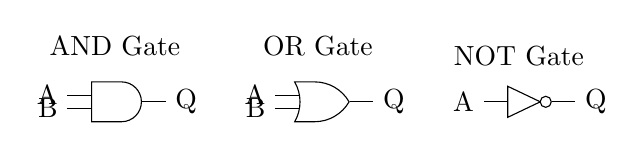
\begin{tikzpicture}[
    gate/.style={draw, thick, minimum width=12mm, minimum height=20mm},
    node distance=20mm
]

% AND Gate
\node[and gate US, draw] (and) {};
\draw (and.input 1) -- ++(-0.3,0) node[left] {A};
\draw (and.input 2) -- ++(-0.3,0) node[left] {B};
\draw (and.output) -- ++(0.3,0) node[right] {Q};

% OR Gate (positioned to the right of AND gate)
\node[or gate US, draw, right=of and] (or) {};
\draw (or.input 1) -- ++(-0.3,0) node[left] {A};
\draw (or.input 2) -- ++(-0.3,0) node[left] {B};
\draw (or.output) -- ++(0.3,0) node[right] {Q};

% NOT Gate (positioned to the right of OR gate)
\node[not gate US, draw, right=of or] (not) {};
\draw (not.input) -- ++(-0.3,0) node[left] {A};
\draw (not.output) -- ++(0.3,0) node[right] {Q};

% Labels
\node[above=2mm] at (and.north) {AND Gate};
\node[above=2mm] at (or.north) {OR Gate};
\node[above=2mm] at (not.north) {NOT Gate};

\end{tikzpicture}
\caption{Basic logic gates with standard symbols and labels.}
\label{fig:logic_gates}
\end{figure}

\textbf{Gates with Multiple Inputs}
\begin{itemize}
    \item \text{Three-input AND Gate:} Outputs $1$ if all inputs are $1$.
    \item \text{Four-input OR Gate:} Outputs $1$ if any input is $1$; outputs $0$ only if all inputs are $0$.
\end{itemize}

\end{document}

